\chapter{El Tarot 650 en Gazebo}
\label{cap:tarot650}

\begin{enpocas}
De dónde sale el vehículo de la simulación, qué se le agregó para que lo vuele PX4, cuáles de sus datos
son supuestos y cómo se cambian por los del dron real, cómo es su variante para ArduPilot y cómo volar
todavía con el x500 de las primeras corridas.
\end{enpocas}

\section{El tarot650\_busqueda}

El vehículo es el \textbf{Tarot Ironman 650}. Su modelo de Gazebo, \cod{tarot650_busqueda}, lo arma
\cod{scripts/generar_vehiculo.py} con dos fuentes:
\begin{itemize}
  \item \textbf{Del Tarot:} las mallas de su CAD (placas, brazos, motores, tren de aterrizaje y hélices,
        carpeta \cod{models/tarot650_busqueda/meshes}), la masa, las inercias, la posición de los
        rotores, las hélices y los motores. Todo sale de la tabla \cod{VEHICULOS['tarot650']} de
        \cod{cuadrirotor_sim/scripts/generar_modelo.py}, otro paquete del mismo \emph{workspace}, así
        que los dos proyectos usan el mismo dron.
  \item \textbf{Del x500 de PX4:} los sensores (IMU, barómetro, magnetómetro y GPS, con el ruido de PX4)
        y con los mismos nombres, porque el puente de PX4 con Gazebo los busca así.
\end{itemize}
Además, \cod{generar_vehiculo.py} pone los motores en el orden de PX4 (\cod{rotor_0} adelante-derecha
antihorario, \cod{rotor_1} atrás-izquierda antihorario, \cod{rotor_2} adelante-izquierda horario,
\cod{rotor_3} atrás-derecha horario), que es también el de las salidas 1--4 de ArduPilot en un ``X'', y
le agrega:
\begin{enumerate}
  \item \textbf{La cámara 24~cm debajo del centro}, justo bajo los patines, mirando hacia abajo
        (la \cod{mono_cam} de PX4: $1280\times960$, campo horizontal de 1.74~rad).
  \item \textbf{Viento habilitado} en el cuerpo (\cod{<enable_wind>}), para que el sistema
        \cod{WindEffects} del mundo lo empuje.
  \item \textbf{Un LiDAR 3D} (360°$\times$120 haces, 16 canales de $-35$° a $+15$°, 30~m, 10~Hz,
        \cod{/dron/lidar/points}) para la evasión de obstáculos.
\end{enumerate}

\begin{table}[H]
\centering\small
\begin{tabular}{ll}
\toprule
\textbf{Parámetro} & \textbf{Valor} \\ \midrule
Masa total & 2.25~kg (cuerpo 2.12, rotores $4\times20$~g, cámara 50~g) \\
Inercia del cuerpo & diag(0.0304, 0.0321, 0.0585)~kg\,m$^2$ \\
Inercia con los rotores & diag(0.0341, 0.0361, 0.0660)~kg\,m$^2$ \\
Rotores & $(\pm0.2198, \pm0.212)$~m, 4~cm sobre el centro, hélices de 15'' \\
$k_f$, $k_m$, $\omega_{max}$ & $4.24\times10^{-5}$~N/(rad/s)$^2$, 0.016~m, 680~rad/s \\
Empuje máximo & 19.6~N por motor, $\approx$3.6 veces el peso en total \\
Vuelo estacionario & $\omega_h = 361$~rad/s por motor \\
Constantes de tiempo de los motores & 0.03~s al subir, 0.05~s al bajar \\
Cámara & $1280\times960$, HFOV 1.74~rad, hacia abajo, $t_{BC} = (0, 0, -0.24)$~m \\
Centro de masa & corrido 0.67~mm en $x$ y en $y$ por la cámara \\
\bottomrule
\end{tabular}
\caption{Parámetros del Tarot 650 de la simulación (\cod{models/tarot650_busqueda/model.sdf} y la tabla
\cod{VEHICULOS} de \cod{codigo/nn_imitacion.py}). Los de masa, inercias, $k_f$ y motores son supuestos.}
\end{table}

El \emph{airframe} de PX4 es \cod{px4/4100_gz_tarot650_busqueda}. Además de la geometría de los rotores
(\cod{CA_ROTOR*}), fija las salidas a los motores de Gazebo entre 100 y 680~rad/s
(\cod{SIM_GZ_EC_MIN}, \cod{SIM_GZ_EC_MAX}), el empuje de vuelo estacionario (\cod{MPC_THR_HOVER} 0.25,
con \cod{THR_MDL_FAC} 0.8) y los parámetros del modo \emph{Neural Control} para la red del Tarot
(\cod{MC_NN_THRST_COEF} 17.0754, \cod{MC_NN_MIN_RPM} 955, \cod{MC_NN_MAX_RPM} 6494; capítulo
\ref{cap:control-neuronal}).

\begin{tecnico}
¿De dónde sale \cod{MPC_THR_HOVER} = 0.25? En vuelo estacionario, $\omega_h = 361$~rad/s. La salida
normalizada del motor es $(361-100)/580 = 0.45$ y, con la curva $0.8x^2 + 0.2x$ que PX4 deshace con
\cod{THR_MDL_FAC} = 0.8, el empuje normalizado es $0.8(0.45)^2 + 0.2(0.45) \approx 0.25$.
\end{tecnico}

\section{Supuestos que hay que reemplazar}

\begin{aviso}
La masa, las inercias, $k_f$ y los retardos de los motores del Tarot de la simulación son
\textbf{supuestos}: no se midieron en un dron real. Las mallas dan la forma, no la física. Antes de
llevar la red neuronal o las ganancias a un Tarot real hay que reemplazarlos por los de ese dron.
\end{aviso}

Los pasos, en orden:
\begin{enumerate}
  \item Mide la masa (con batería, cámara y todo lo que vaya a volar), las inercias, $k_f$ y $k_m$ (en
        un banco de empuje) y la respuesta de los motores.
  \item Ponlos en la tabla \cod{VEHICULOS['tarot650']} de \cod{cuadrirotor_sim/scripts/generar_modelo.py}
        y en la de \cod{codigo/nn_imitacion.py}, y vuelve a generar el vehículo
        (\cod{python3 scripts/generar_vehiculo.py}).
  \item Si cambian la posición de los rotores, $\omega_{max}$ o el empuje de vuelo estacionario, ajusta el
        \emph{airframe} \cod{px4/4100_gz_tarot650_busqueda} y \cod{config/ardupilot/tarot650.parm}.
  \item Reentrena la red (\cod{nn_imitacion.py --vehiculo tarot650 --masa ... --com ...}), expórtala e
        instálala en PX4 (capítulo~\ref{cap:instalacion}).
\end{enumerate}

\section{La variante para ArduPilot}

\cod{tarot650_busqueda_ardupilot} es el mismo vehículo con:
\begin{itemize}
  \item \cod{ArduPilotPlugin}, que intercambia sensores y motores con ArduCopter (salidas de
        1000--2000~µs $\rightarrow$ 0--680~rad/s, mismo orden de motores que PX4);
  \item una IMU para ArduPilot, con ruido y sesgo supuestos (giróscopo 0.004~rad/s, acelerómetro
        0.1~m/s$^2$), y \cod{OdometryPublisher} a 400~Hz (el estado para la red);
  \item \cod{no_time_sync=0}, para que ArduPilot vuele con su EKF3 y no con el estado verdadero del
        simulador (capítulo~\ref{cap:pilotos});
  \item el sistema \cod{SelectorMotores} (paquete \cod{mision_gz_plugins}), que deja pasar los comandos
        de ArduPilot o los de la red, según lo que pida la misión.
\end{itemize}
En esa variante el vehículo va dentro del mundo, que corre a 1~kHz (lo que espera ArduPilot). Sus
parámetros de vuelo están en \cod{config/ardupilot/tarot650.parm}: salidas de 1000--2000~µs con curva
de empuje cuadrática pura (\cod{MOT_THST_EXPO} 1.0), \cod{MOT_THST_HOVER} 0.28 ($(361/680)^2$), lazos
de tasa más suaves que los del Iris (el Tarot tiene motores más lentos) y \cod{AHRS_EKF_TYPE} 3.

\begin{lstlisting}[style=bash]
python3 scripts/generar_vehiculo.py      # escribe models/tarot650_busqueda, models/x500_busqueda y sus variantes _ardupilot
bash scripts/instalar_px4.sh ~/ros2_ws/src/mision/codigo/control_net_tarot650_busqueda    # y los copia a PX4
\end{lstlisting}

\section{El x500 de PX4 sigue disponible}

Las primeras corridas, las del 22 y el 23 de octubre, se hicieron con el \textbf{x500} de PX4, y varias
cifras del libro vienen de ellas. El vehículo sigue en el paquete y se elige con un argumento:
\begin{lstlisting}[style=bash]
ros2 launch mision simulacion.launch.py vehiculo:=x500
\end{lstlisting}
\cod{x500_busqueda} parte del \cod{x500_mono_cam_down} de PX4 con los mismos tres cambios (cámara bajo los
patines, viento y LiDAR); usa el \emph{airframe} \cod{4099_gz_x500_busqueda}, \cod{config/ardupilot/x500.parm}
y la red \cod{pesos_nn_x500_busqueda.npz} / \cod{control_net_x500_busqueda}.

\begin{figure}[H]
\centering
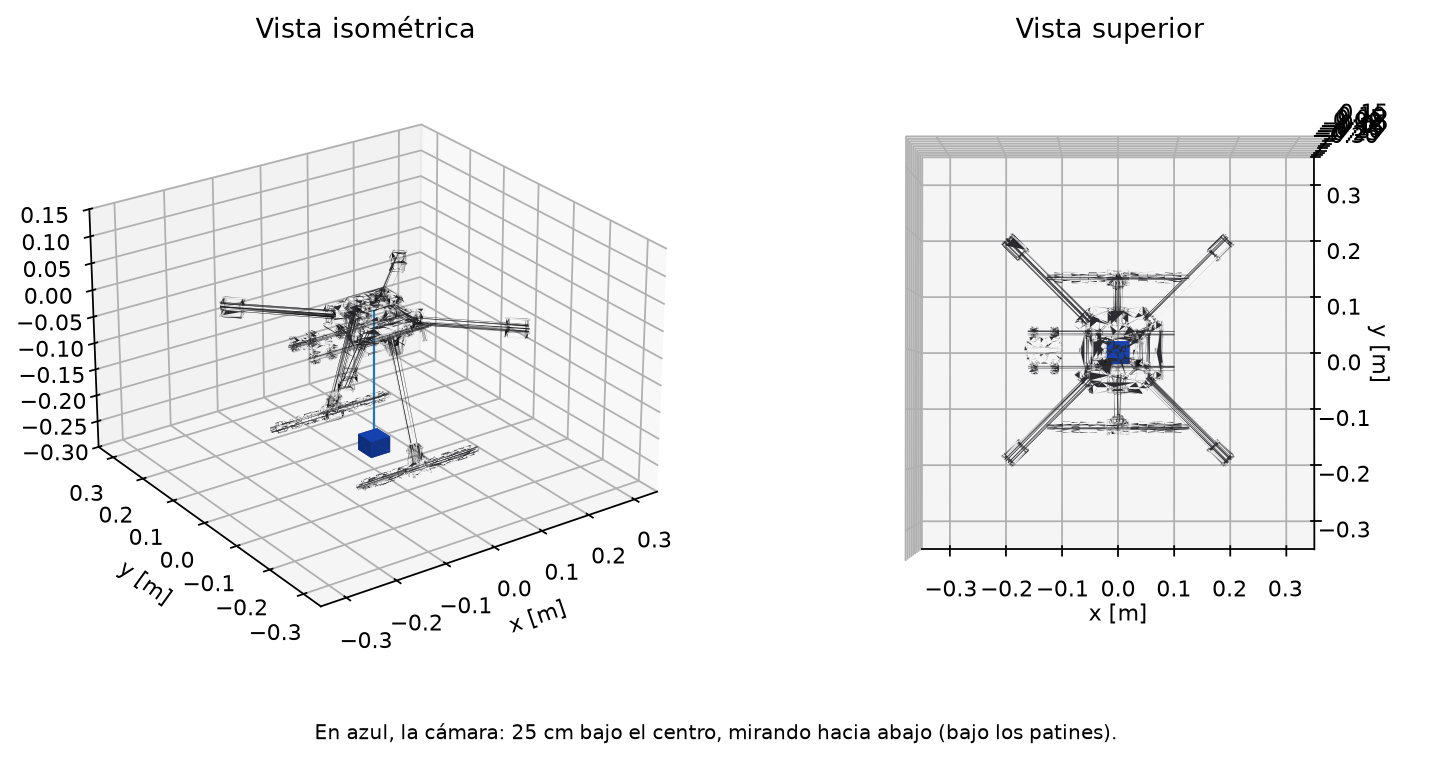
\includegraphics[width=0.85\textwidth]{x500_render.png}
\caption{El x500 de PX4, dibujado a partir de las mallas de su modelo.}
\end{figure}

\begin{table}[H]
\centering\small
\begin{tabular}{ll}
\toprule
\textbf{Parámetro} & \textbf{Valor} \\ \midrule
Masa total & 2.114~kg (cuerpo 2.0, rotores $4\times16$~g, cámara 50~g) \\
Inercia del cuerpo & diag(0.0217, 0.0217, 0.040)~kg\,m$^2$ \\
Rotores & $(\pm0.174, \pm0.174)$~m, hélices de 13'' \\
$k_f$, $k_m$, $\omega_{max}$ & $8.54858\times10^{-6}$~N/(rad/s)$^2$, 0.016~m, 1000~rad/s \\
Constantes de tiempo de los motores & 12.5~ms al subir, 25~ms al bajar \\
Cámara & $1280\times960$, HFOV 1.74~rad, hacia abajo, $t_{BC} = (0, 0, -0.25)$~m \\
Centro de masa & corrido 0.7~mm en $x$ y en $y$ por la cámara \\
\bottomrule
\end{tabular}
\caption{Parámetros del x500 de la simulación.}
\end{table}

\begin{leccion}
En el modelo de PX4 la cámara está 10~cm \emph{arriba} del centro y mira hacia abajo a través del
cuerpo: el armazón, los motores y el tren de aterrizaje tapaban más de la mitad de la imagen. El diseño
original suponía 10~cm \emph{abajo}. En el x500 la cámara se movió 25~cm abajo y en el Tarot va 24~cm
abajo; el localizador usa el valor de cada vehículo ($t_{BC}$, parámetro \cod{z_camara} que le pasa
el \emph{launch}).
\end{leccion}

\begin{aviso}
PX4 lleva una sola red compilada, y ahora es la del Tarot. Para volar el x500 con \cod{controlador:=red}
en PX4 hay que reinstalar la suya:
\cod{bash scripts/instalar_px4.sh ~/ros2_ws/src/mision/codigo/control_net_x500_busqueda}. Con ArduPilot
no hace falta: \cod{controlador_red} carga los pesos del vehículo que se lanza.
\end{aviso}

\section{Las personas}

Cuatro modelos de OpenRobotics (Gazebo Fuel, CC0): de pie, caminando, mujer y sentada (Rescue Randy),
todos estáticos y con la etiqueta~1 del sistema \cod{Label}. La persona acostada es uno de pie girado
90°. Los copia y adapta \cod{scripts/importar_personas.py}.

\begin{figure}[H]
\centering
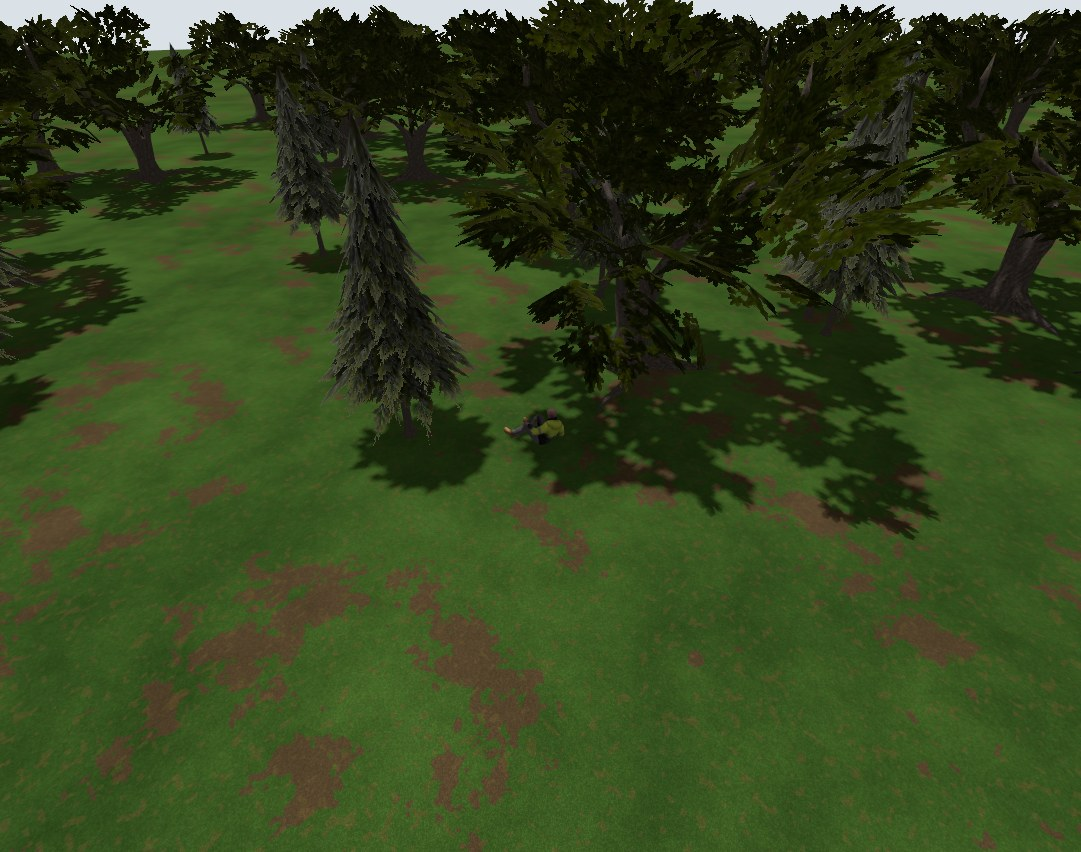
\includegraphics[width=0.6\textwidth]{gz_persona_sentada.jpg}
\caption{Una persona sentada bajo los árboles: desde arriba, una copa puede taparla por completo.}
\end{figure}
